\documentclass[10pt, a4j, dvipdfmx]{jarticle}
\usepackage{titlesec}
\usepackage[dvipdfmx]{graphicx}
\usepackage[dvipdfmx]{color}
\usepackage{float}
\usepackage{wrapfig}
\usepackage{subfigure}
\usepackage{caption}

\makeatletter
\newcommand{\figcaption}[1]{\def\@captype{figure}\caption{#1}}
\newcommand{\tblcaption}[1]{\def\@captype{table}\caption{#1}}
\makeatother

\title{双安定マルチバイブレータ}
\author{4年 電子システム工学科 40番  山地 駿徹}


\begin{document}
    \section{目的}
    トランジスタを用いた双安定マルチバイブレータを設計・制作し,外部からトリガパルスを周期的に入力したときの各部の波形を測定して,回路の動作を明確に理解することを目的とする.

    \section{原理}
    \begin{wrapfigure}{r}{70mm}
        \vspace*{-\intextsep}
        \begin{center}
        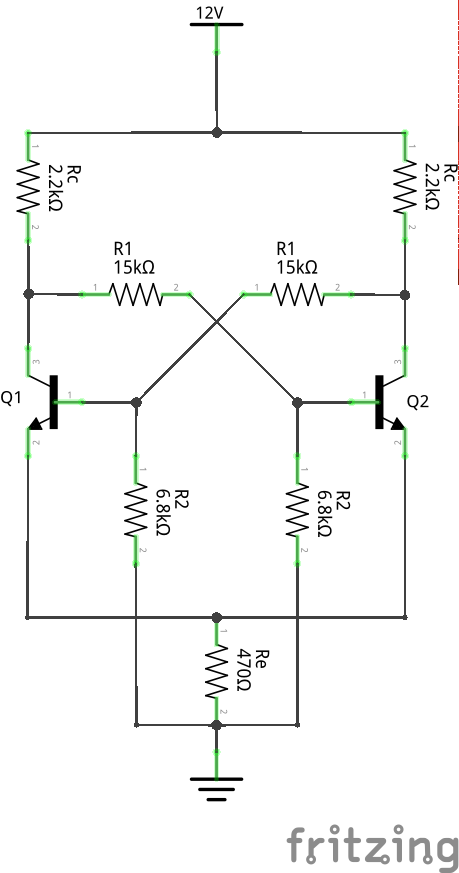
\includegraphics[height=40mm]{images/fig-1.png}
        \caption{セルフバイアス型双安定マルチバイブレータ}
        \label{fig:1}
        \end{center}
    \end{wrapfigure}
       
    セルフバイアス型双安定マルチバイブレータの回路を図\ref{fig:1}に示す.

    \paragraph{2つの安定状態}
    双安定マルチバイブレータには,次の2つの安定な状態がある.\\
    \begin{tabular}{ll}
        安定状態1 & トランジスタQ1がOFF\\
         & トランジスタQ2がON \\
        安定状態2 & トランジスタQ1がON \\
         & トランジスタQ2がOFF \\
    \end{tabular}

    \paragraph{回路解析}
    図\ref{fig:1}に示すセルフバイアス型双安定マルチバイブレータにおいて、トランジスタQ1がOFFでトランジスタQ2がONの安定な状態にあるとする.

    トランジスタQ2のコレクタとアース間にかかるテブナン電圧と図テブナン抵抗を求める.
    テブナン電圧$E_{C2}$は,図\ref{fig:2}の回路から次の式のように求めることができる.
    \begin{eqnarray}
        \{(R_1 + R_2) / (R_1 + R_2 + R_C)\} \cdot V_{CC} & = & \{(15 + 6.8) / (15 + 6.8 + 2.2)\} * 12 \nonumber \\  
        & = & 10.90 [V] \nonumber
    \end{eqnarray}
    テブナン抵抗$R_{C2}$は,
    \begin{eqnarray}
        \{(R_1 + R_2) \cdot R_C / (R_1 + R_2 + R_C) \} & = & (15 + 6.8) \times 2.2 / (15 + 6.8 + 2.2) \nonumber \\
        & = & 2.00 [k\Omega] \nonumber
    \end{eqnarray}

    \begin{figure}[H]
        \begin{minipage}{0.5\hsize}
            \centering
            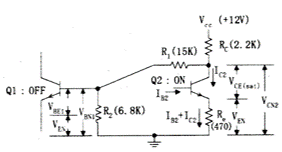
\includegraphics[height=50mm]{images/fig-2.png}
            \caption{TrQ1のベースとTrQ2のコレクタの接続図}
            \label{fig:2}
        \end{minipage}
        \begin{minipage}{0.5\hsize}
            \centering
            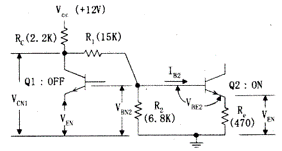
\includegraphics[height=50mm]{images/fig-3.png}
            \caption{TrQ1のベースとTrQ2のコレクタの接続図}
            \label{fig:3}
        \end{minipage}
    \end{figure}

    トランジスタQ2のベースとアース間にかかるテブナン電圧とテブナン抵抗を求める.
    テブナン電圧$E_{B2}$は,図\ref{fig:3}の回路から次の式のように求めることができる.
    \begin{eqnarray}
        \{R_2 / (R_1 + R_2 + R_C)\} \cdot V_{CC} & = & \{6.8 / (15 + 6.8 + 2.2)\} \times 12 \nonumber \\
        & = & 3.40 [V] \nonumber
    \end{eqnarray}
    テブナン抵抗$R_{B2}$は,
    \begin{eqnarray}
        (R_1 + R_C) \cdot R_2 / (R_1 + R_2 + R_C) & = & (15 + 2.2) \times 6.8 / (15 + 6.8 + 2.2) \nonumber \\
        & = & 4.87 [k\Omega] \nonumber
    \end{eqnarray}
    トランジスタQ2のコレクタおよびベース端子にかかるテブナン電圧とテブナン抵抗が求まったので,トランジスタQ2側は図\ref{fig:4}の回路と等価である.
    図\ref{fig:4}の回路のベース側をコレクタ側の閉回路において,次の式が成り立つ.
    \begin{eqnarray}
        R_{B2} \cdot I_{B2} + R_e (I_{B2} + I_{C2}) = E_{B2} - V_{BE(sat)} \nonumber \\
        R_{C2} \cdot I_{C2} + R_e (I_{B2} + I_{C2}) = E_{C2} - V_{CE(sat)} \nonumber
    \end{eqnarray}
    値を代入すると,
    \begin{eqnarray}
        4.87 \times I_{B2} + 0.47 \times (I_{B2} + I_{C2}) = 3.40 - 0.7 \nonumber \\
        2.00 \times I_{C2} + 0.47 \times (I_{B2} + I_{C2}) = 10.90 - 0.2 \nonumber
    \end{eqnarray}
    この連立方程式を解くと,次のように求まる.
    \begin{eqnarray}
        I_{B2} = 126 [\mu A] \nonumber \\
        I_{C2} = 4.31 [mA] \nonumber
    \end{eqnarray}
    \begin{wrapfigure}{r}{70mm}
        \vspace*{-\intextsep}
        \begin{center}
        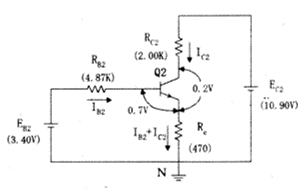
\includegraphics[height=40mm]{images/fig-4.png}
        \caption{非安定マルチバイブレータ}
        \label{fig:4}
        \end{center}
    \end{wrapfigure}
    この安定状態1におけるトランジスタQ2の$h_{FE}$は,
    \[
        h_{FE} = I_{C2} / I_{B2} = 34.2
    \]
    となり,能動領域のトランジスタQ2の$h_{FE}$が100前後なので,トランジスタQ2は過飽和領域にあることが分かる.
    抵抗$R_e$における電圧降下$V_{EN}$は,
    \[
        V_{EN} = 0.47 \times (0.126 + 4.31) = 2.08 [V]
    \]
    トランジスタQ2のコレクタ電位は,$V_{CE_{sat}} = 0.2 [V]$とすると,
    \[
        V_{CN2} = V_{CE2} + V_{EN} = 0.2 + 2.08 = 2.28 [V]
    \]
    トランジスタQ2のベース電位は,
    \[
        V_{BN2} = V_{BE2} + V_{EN} = 0.6 + 2.08 = 2.68 [V]
    \]
    トランジスタQ1のベース電位は,
    \[
        V_{BN1} = V_{CN2} + R_2 / (R_1 + R_2) = 0.71 [V]
    \]
    トランジスタQ1のベースエミッタ間の電圧は,
    \[
        V_{BE1} = V_{BN1} - V_{EN} = 0.71 - 2.08 = -1.37 [V] < 0 [V] (Tr Q1 : OFF)
    \]
    したがって,トランジスタQ1は遮断領域にあることが分かる.
    トランジスタQ1のコレクタ電位は,
    \[
        V_{CN1} = V_{CC} \cdot R_1 / (R_C + R_1) + V_{BN2} \cdot R_C / (R_C + R_1) = 10.81 [V]
    \]
    となる.以上のことから,安定状態1における各部の電圧と電流は,

    \begin{minipage}{0.5\hsize}
        \begin{eqnarray}
            I_{C1} = 0 [mA] \nonumber \\
            I_{B1} = 0 [\mu A] \nonumber \\
            V_{CN1} = 10.81 [V] \nonumber \\
            V_{BN1} = 0.71 [V] \nonumber \\
            V_{BE1} = -1.37 [V] \nonumber \\
            V_{EN} = 2.08 [V] \nonumber
        \end{eqnarray}
    \end{minipage}
    \begin{minipage}{0.5\hsize}
        \begin{eqnarray}
            I_{C2} = 0 [mA] \nonumber \\
            I_{B2} = 126 [\mu A] \nonumber \\
            V_{CN2} = 2.28 [V] \nonumber \\
            V_{BN2} = 2.68 [V] \nonumber \\
            V_{BE2} = 0.7 [V] \nonumber
        \end{eqnarray}
    \end{minipage}

    となる.外部からトランジスタQ2のベースに負のトリガパルスが入力されると,トランジスタQ2がOFF,トランジスタQ1がONになり安定状態2となる.
    トランジスタQ1とQ2の特性が同じだと仮定すると,安定状態2における各部の電圧と電流は,

    \begin{minipage}{0.5\hsize}
        \begin{eqnarray}
            I_{C1} = 4.31 [mA] \nonumber \\
            I_{B1} = 126 [\mu A] \nonumber \\
            V_{CN1} = 2.28 [V] \nonumber \\
            V_{BN1} = 2.68 [V] \nonumber \\
            V_{BE1} = 0.7 [V] \nonumber \\
            V_{EN} = 2.08 [V] \nonumber
        \end{eqnarray}
    \end{minipage}
    \begin{minipage}{0.5\hsize}
        \begin{eqnarray}
            I_{C2} = 0 [mA] \nonumber \\
            I_{B2} = 0 [\mu A] \nonumber \\
            V_{CN2} = 10.82 [V] \nonumber \\
            V_{BN2} = 0.71 [V] \nonumber \\
            V_{BE2} = -1.37 [V] \nonumber
        \end{eqnarray}
    \end{minipage}

    となる.このことから,この双安定マルチバイブレータのスイング幅は,
    \[
        10.81 - 2.28 = 8.53 [V]
    \]
    となる.

    \paragraph{正帰還作用による反転動作}
    \begin{wrapfigure}{r}{70mm}
        \vspace*{-\intextsep}
        \begin{center}
        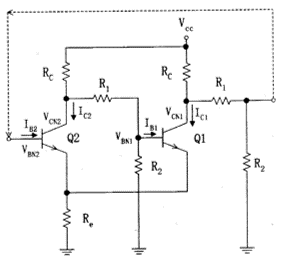
\includegraphics[height=40mm]{images/fig-5.png}
        \caption{二段増幅回路の働き(正帰還)}
        \label{fig:5}
        \end{center}
    \end{wrapfigure}
    トランジスタQ1がOFF,トランジスタQ2がONの安定状態1にあるとき,トランジスタQ2のベースに負のトリガパルスが入力されたときの動作を考える.

    Q2のベースに負のトリガパルスが加えられた瞬間,$V_{BE2} < 0 [V]$となり,トランジスタQ2はOFFとなる.
    トランジスタQ2がOFFになると,トランジスタQ2のコレクタ電位$V_{CN2}$が$V_{CC}$の値に近づく.$V_{CN2}$が高くなると,相対的にトランジスタQ1のベース電位$V_{BN1}$が高くなり,$V_{BE1} > 0.6[V]$となり,トランジスタQ1がON状態になる.
    Q1がONになるとトランジスタQ1のコレクタ電流$I_{C1}$が流れQ1のコレクタ電位$V_{CN1}$は低くなる.$V_{CN1}$が下がると相対的にトランジスタQ2のベース電位$V_{BN2}$も下がり,Q2のベースエミッタ間電圧$V_{BE2}$が小さくなる.
    $V_{BE2}$が小さくなるとトランジスタQ2もベース電流$I_{B2}$は減少し,コレクタ電流$I_{C2}$も減少し,コレクタ電位$V_{CN2}$はより高くなる.
    この正帰還作用が繰り返され,最終的にトランジスタQ1がON(飽和領域),トランジスタQ2がOFF(遮断領域)の安定状態2となる.

    トランジスタQ1がON,トランジスタQ2がOFFの安定状態2にあるとき,トランジスタQ1のベースに負のトリガパルスが入力されると同じように正帰還作用が働きトランジスタQ1がOFF,トランジスタQ2がONの安定状態1になる.

    \paragraph{スピードアップコンデンサの働き}
    \begin{wrapfigure}{r}{70mm}
        \vspace*{-\intextsep}
        \begin{center}
        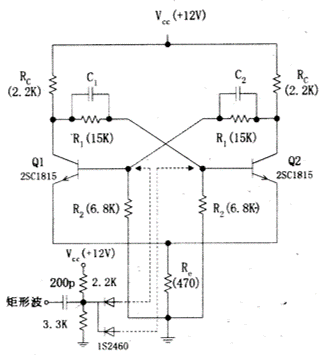
\includegraphics[height=40mm]{images/fig-6.png}
        \caption{セルフバイアス型双安定マルチバイブレータ}
        \label{fig:6}
        \end{center}
    \end{wrapfigure}
    図\ref{fig:6}の回路において,トリガパルスが入力されると,一瞬トランジスタQ1とQ2はともにOFFとなる.
    トリガパルスが入力される前の状態が,トランジスタQ1がOFFでトランジスタQ2がONの安定状態1であったとする.このとき,コンデンサ$C_1 = 8.05[V]$,$C_2 = 1.67[V]$の電圧がかかっている.

    トリガパルスが入力されると,トランジスタQ2のコレクタ電位は$V_{CN2} = 2.37 [V]$から$V_{CN2} = 10.9 [V]$ になる.
    その瞬間,トランジスタQ1のベース電位は$V_{VB1} = 2.77 [V]$から$V_{BN1} = 10.9 - 8.05 = 2.85 [V]$に引き上げられる.このとき,トランジスタQ1とQ2はともに飽和領域にあるが,トランジスタQ1のほうがQ2に比べはるかに過飽和の状態にある.

    一瞬後,負のパルスがなくなった瞬間,$V_{BN1} = 9.32[V]$,$V_{BN2} = 2.77[V]$になり,トランジスタQ1は過飽和領域にあり$V_{CN1} = 0.2 [V]$となり,$V_{BN2} = 0.2 - 8.05 = -7.85[V]$となり,トランジスタQ2はOFFとなる.
    すなわち,トランジスタQ1がONでトランジスタQ2がOFFの安定状態2となる.

    もし,スピードアップコンデンサがなければ,負のパルスが入った瞬間トランジスタQ1とQ2はともにOFFとなり,$V_{CN1} = V_{CN2} = 10.9[V]$,$V_{BN1} = V_{BN2} = 3.40[V]$となり,トランジスタQ1とQ2はONとなり,トランジスタの特性や抵抗値の誤差などから一方がONで他方がOFFとなる.次のトリガパルスが入っても同じ現象が起こり,ONになり易いほうが常にONとなり,状態が反転しない.

    スピードアップコンデンサは,充電されている電圧の違いによって前の安定状態を記憶しており,次にトリガパルスが加わったとき安定状態の反転を間違いなくやってのける働きを持っている.
    ここでは説明を省略するが名前の示すように,他にもコレクタ電流波形の立ち上がり・立ち下がりを速やかにし,立ち上がり時間.立ち下がり時間を短くする役割をはたす.


    \newpage
    \section{セルフバイアス型双安定マルチバイブレータの設計}
    トランジスタQ1がOFFでトラジスタQ2がONという安定状態2となる条件を考える.

    \paragraph{トランジスタQ2がONになる条件}
    図\ref{fig:4}のトランジスタQ2がONのときの等価回路に於いて,次の式が成り立つ.
    \begin{eqnarray}
        R_{B2} \cdot I_{B2} + R_e (I_{B2} + I_{C2}) = E_{B2} - V_{BE_{(sat)}} \nonumber \\
        R_{C2} \cdot I_{C2} + R_e (I_{B2} + I_{C2}) = E_{C2} - V_{CE_{(sat)}} \nonumber
    \end{eqnarray}
    この連立方程式を$I_{C2}$と$I_{B2}$について解くと
    \begin{eqnarray}
        I_{C2} = \{(E_{C2} - V_{CE_{(sat)}})(R_{B2} + R_e) - (E_{B2} - V_{BE_{(sat)}}) R_e\} / A \nonumber \\
        I_{B2} = \{(E_{B2} - V_{BE_{(sat)}})(R_{C2} + R_e) - (E_{C2} - V_{CE_{(sat)}}) R_e\} / A \nonumber \\
        ここで, A = (R_{C2} + R_e)(R_{B2} + R_e) - R_e^2 \nonumber
    \end{eqnarray}
    これらの式から,$R_2$に対する$R_1$の上限が得られる.

    \paragraph{トランジスタQ1がOFFになる条件}
    図\ref{fig:2}において,次の関係が成り立つ.
    \begin{eqnarray}
        I_2 = I_{CBO} + I_1 \nonumber \\
        V_{BN1} & = & R_2 I_2 \nonumber \\
        & = & V_{EN} + V_{CE_{(sat)}} - R_1 I_1 \nonumber \\
        & = & V_{EN} + V_{CE_{(sat)}} - R_1 (I_2 - I_{CBO}) \nonumber \\
    \end{eqnarray}
    したがって,
    \[
        I_2 = (V_{EN} + V_{CE_{(sat)}} + R_1 I_{CBO}) / (R_1 + R_2)
    \]
    トランジスタQ1がOFFになるためには
    \[
        V_{BN1} \leq (V_{EN} + V_{CE_{(sat)}} + R_1 I_{CBO}) \cdot R_2 / (R_1 + R_2)
    \]
    よって,$R_2$に対する$R_1$の下限は
    \[
        R_1 \leq  R_2 \cdot (V_{EN} + V_{CN_{(sat)}} - V_{BN1}) / (V_{BN1} - R_2 I_{CBO})
    \]
    \newpage
    \begin{wrapfigure}{r}{70mm}
        \vspace*{-\intextsep}
        \begin{center}
        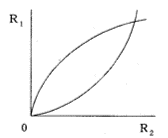
\includegraphics[height=40mm]{images/fig-7.png}
        \caption{ONとOFFの\\条件を満たすR1とR2の関係}
        \label{fig:7}
        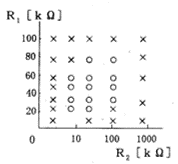
\includegraphics[height=40mm]{images/fig-8.png}
        \caption{動作の範囲}
        \label{fig:8}
        \end{center}
    \end{wrapfigure}
    $V_{BN1}$はカットオフベース電圧である.
    これは$0.5[V]$程度の逆バイアスであるが,実用上では$0[V]$とおいてよい.

    $R_2$に対する$R_1$の上限と下限の式から,図\ref{fig:7}のようなグラフが得られる.
    このグラフの上限と加減に囲まれる範囲の$R_1$と$R_2$を選んで回路を制作する.

    図\ref{fig:7}のグラフを求めることができない場合は,$V_{CC} = 12 [V]$,$R_C = 2.2 [k\Omega]$,$R_e = 470 [\Omega]$,と設定し,$R_2$の値を適当に選び(例えば$R_2 = 6.8 [k\Omega]$),これらの値を上限と下限の式に代入して$R_1$を算出する.


    \newpage
    \section{実験手順}
    \subsection{回路制作}
    図\ref{fig:1}の回路を制作する.
    \subsection{動作の確認}
    手動でQ1のベースとQ2のベースを交互にアースとショートさせることでセット,リセットを行い,Q1とQ2のコレクタ端子をオシロスコープで観測し,安定状態1と安定状態2が交互に移り変わることを確認する.
    \subsection{反転動作の確認}
    図\ref{fig:6}の微分回路をを組み込み,ダイオードを介してベース端子に接続する.発振器の矩形波の出力を微分回路に入力し,マルチバイブレータの動作をオシロスコープで観測する.トリガパルスが入力される度に,マルチバイブレータの安定状態が反転するかどうか調べる.
    \subsection{スピードアップコンデンサの追加と反転動作の確認}
    反転動作がうまく行われないことを確認したならば,スピードアップコンデンサを接続して,今度は反転動作がうまく行われていることを確認する.
    \subsection{分解能周波数の測定}
    スピードアップコンデンサの値を変えて,分解能周波数を測定する.

    \section{使用器具}
    今回の実験において,以下の表に示す器具を用いて測定を行った.
    \begin{figure}[H]
        \centering
        \tblcaption{使用器具}
        \label{tbl:使用器具}
        \begin{tabular}{|c|c|c|}\hline
            使用器具名 & 型番 & 管理番号等 \\\hline
            ディジタルオシロスコープ & DSO3062A & BH43H17S00000021 \\\hline
            多出力直流安定化電源 & PW26-1AT & 20"と書いた黄色いシールのあるもの \\\hline
            直流安定化電源 & PR18-1.2A & い 102 383 \\\hline
            直流電圧計 & 2051-05 & い 54 102 \\\hline
            低周波発振器 & AG-203E & 20"と書いた黄色いシールのあるもの \\\hline
            デジタル・マルチメータ & VOAC86A & 20"と書いた赤いシールのあるもの \\\hline
        \end{tabular}
    \end{figure}

    \newpage
    \section{実験結果}
    \subsection{回路制作}
    以下,図\ref{fig:ex-1}に図\ref{fig:1}の回路図をもとに実際に作成した回路の写真を示す.
    \begin{figure}[H]
        \centering
        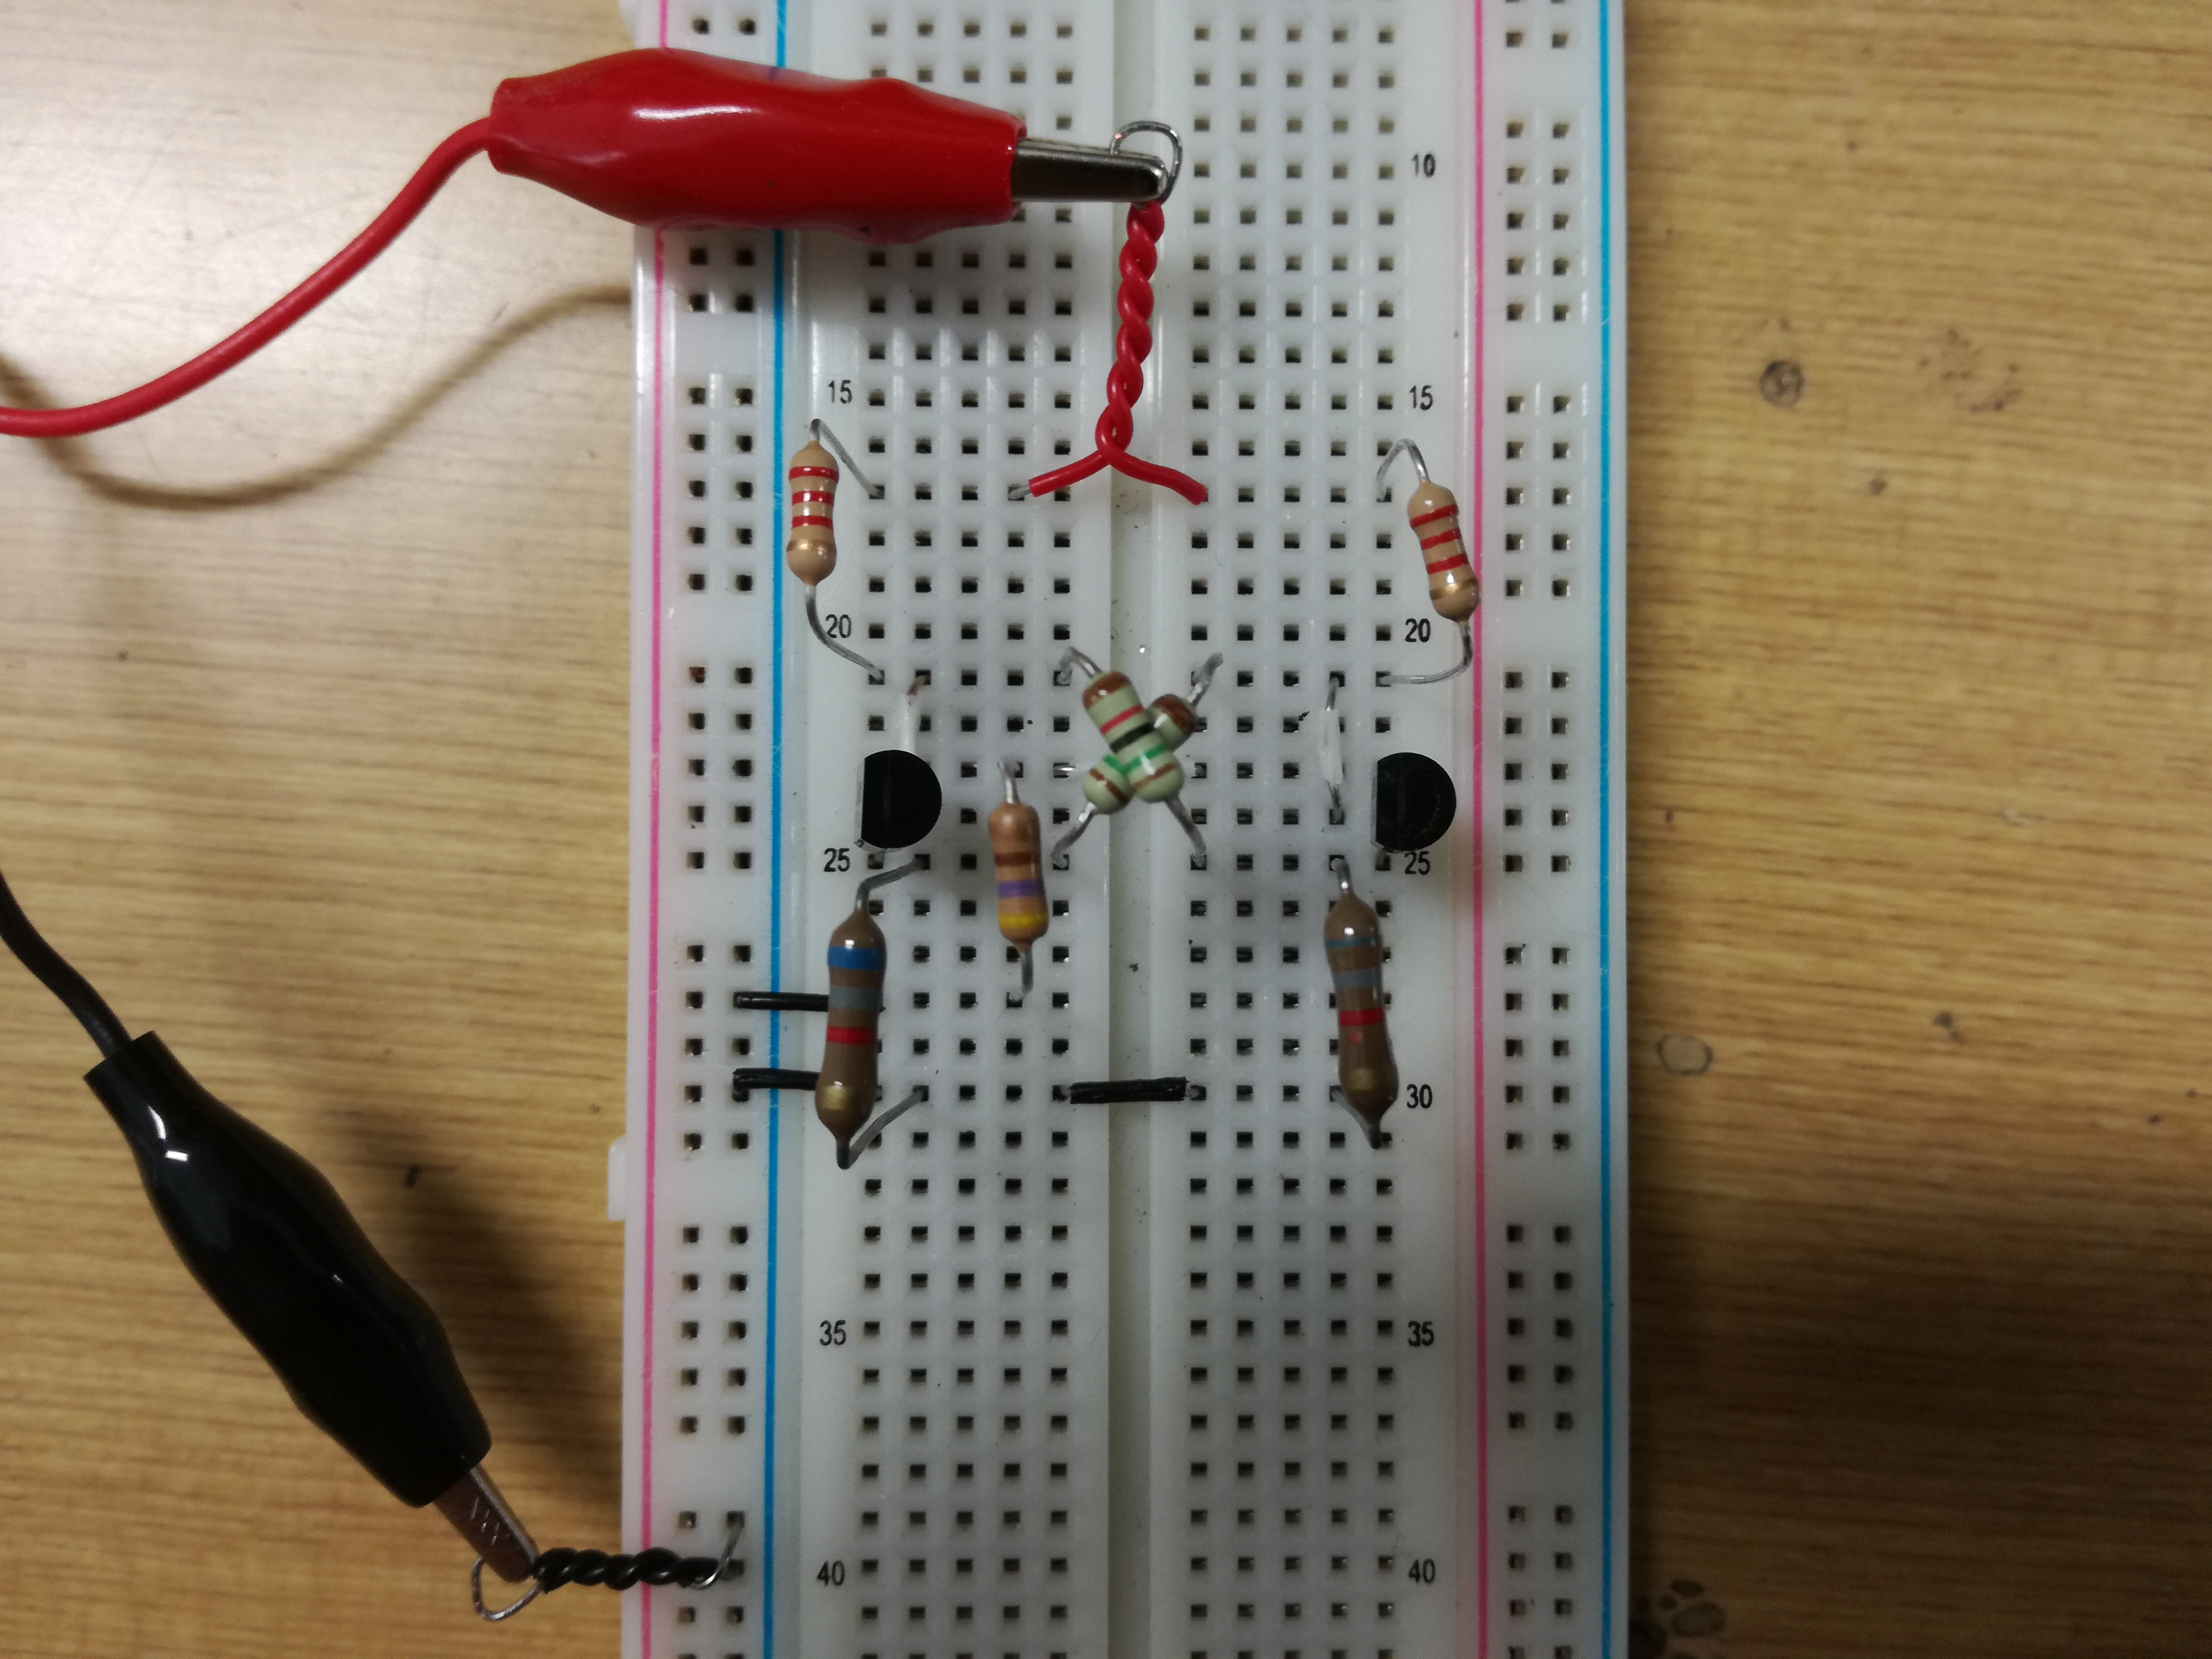
\includegraphics[height=50mm]{images/ex-1.jpg}
        \caption{制作した回路}
        \label{fig:ex-1}
    \end{figure}
    \subsection{動作の確認}
    実験データ紛失のため,測定結果なし.
    \subsection{反転動作の確認}
    実験データ紛失のため,測定結果なし.
    \subsection{スピードアップコンデンサの追加と反転動作の確認}
    実験データ紛失のため,測定結果なし.
    \subsection{分解能周波数の測定}
    6.1に示した回路を用いて,4.5の実験を行った.その測定値を表\ref{tbl:2}に,グラフを図\ref{fig:ex-5}に示す.
    \begin{figure}[H]
        \begin{minipage}{0.5\hsize}
            \centering
            \tblcaption{分解能周波数の測定}
            \label{tbl:2}
            \begin{tabular}{|c|c|}\hline
                静電容量[pF] & 周波数[Hz] \\\hline
                150 & 625000 \\\hline
                220 & 515500 \\\hline
                330 & 420200 \\\hline
                470 & 322600 \\\hline
                680 & 243900 \\\hline
                1000 & 188700 \\\hline
                2200 & 81970 \\\hline
                2700 & 70420 \\\hline
            \end{tabular}
        \end{minipage}
        \begin{minipage}{0.5\hsize}
          \centering
          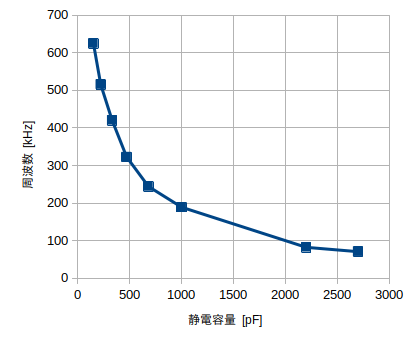
\includegraphics[height=50mm]{images/ex-5.png}
          \caption{測定値のグラフ}
          \label{fig:ex-5}
        \end{minipage}
    \end{figure}
    実験データ紛失のため,波形の測定結果なし.

    \newpage
    \section{考察}
    データの紛失により,実験手順4.2〜4.4までの実験の結果がないため,私が使用できる器具で4.2の実験を再現した.以下にその手順を示す.
    \subsection{実験}
    \subsubsection{実験回路の制作}
    今回測定に際し,オシロスコープが使える状況にいなかったため,ArduinoのAnalog入力を使用して波形の観測を試みることとした.以下,図\ref{fig:自作回路図}に使用した回路図と,図\ref{fig:自作回路写真}に制作した回路の写真を示す.
    \begin{figure}[H]
        \begin{minipage}{0.5\hsize}
            \centering
            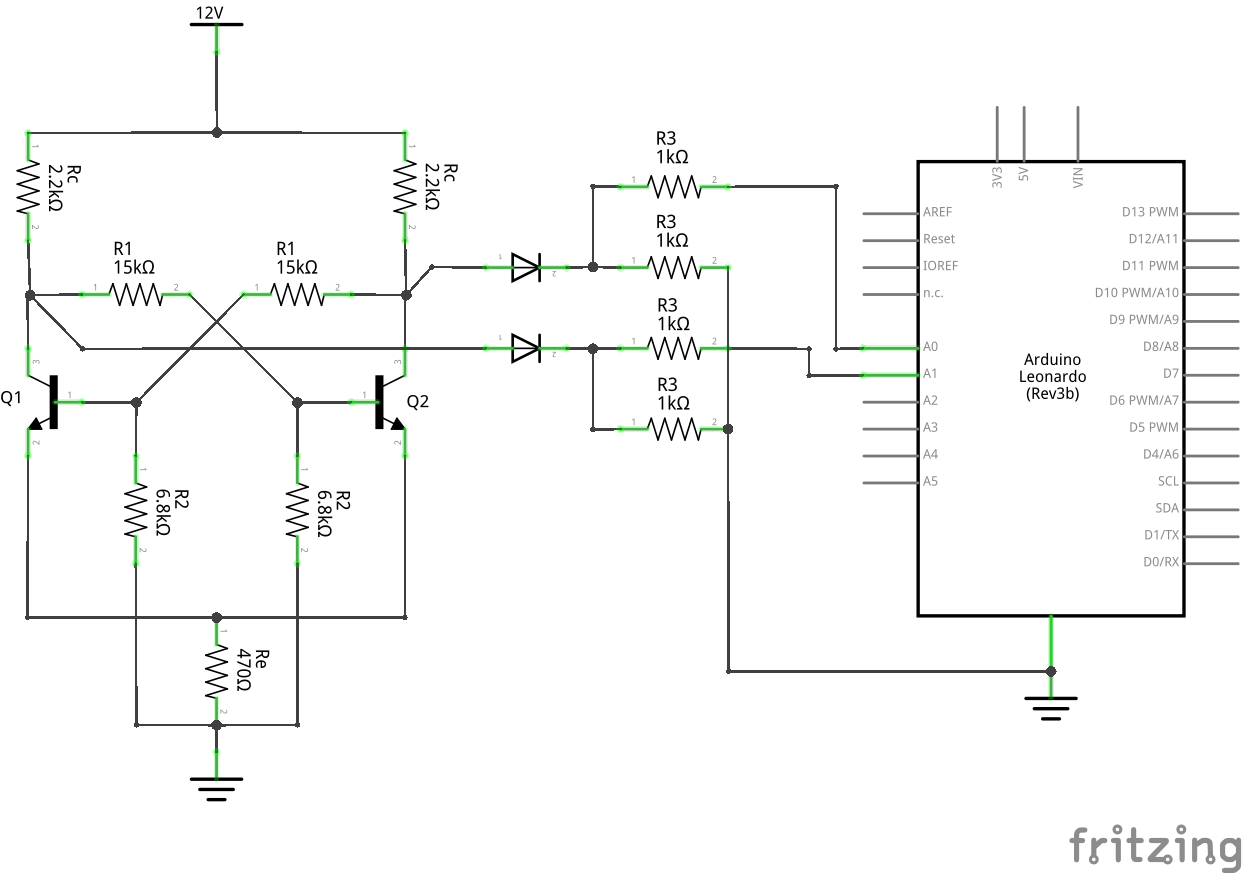
\includegraphics[height=50mm]{images/jisaku-zu.png}
            \caption{回路図}
            \label{fig:自作回路図}
        \end{minipage}
        \begin{minipage}{0.5\hsize}
            \centering
            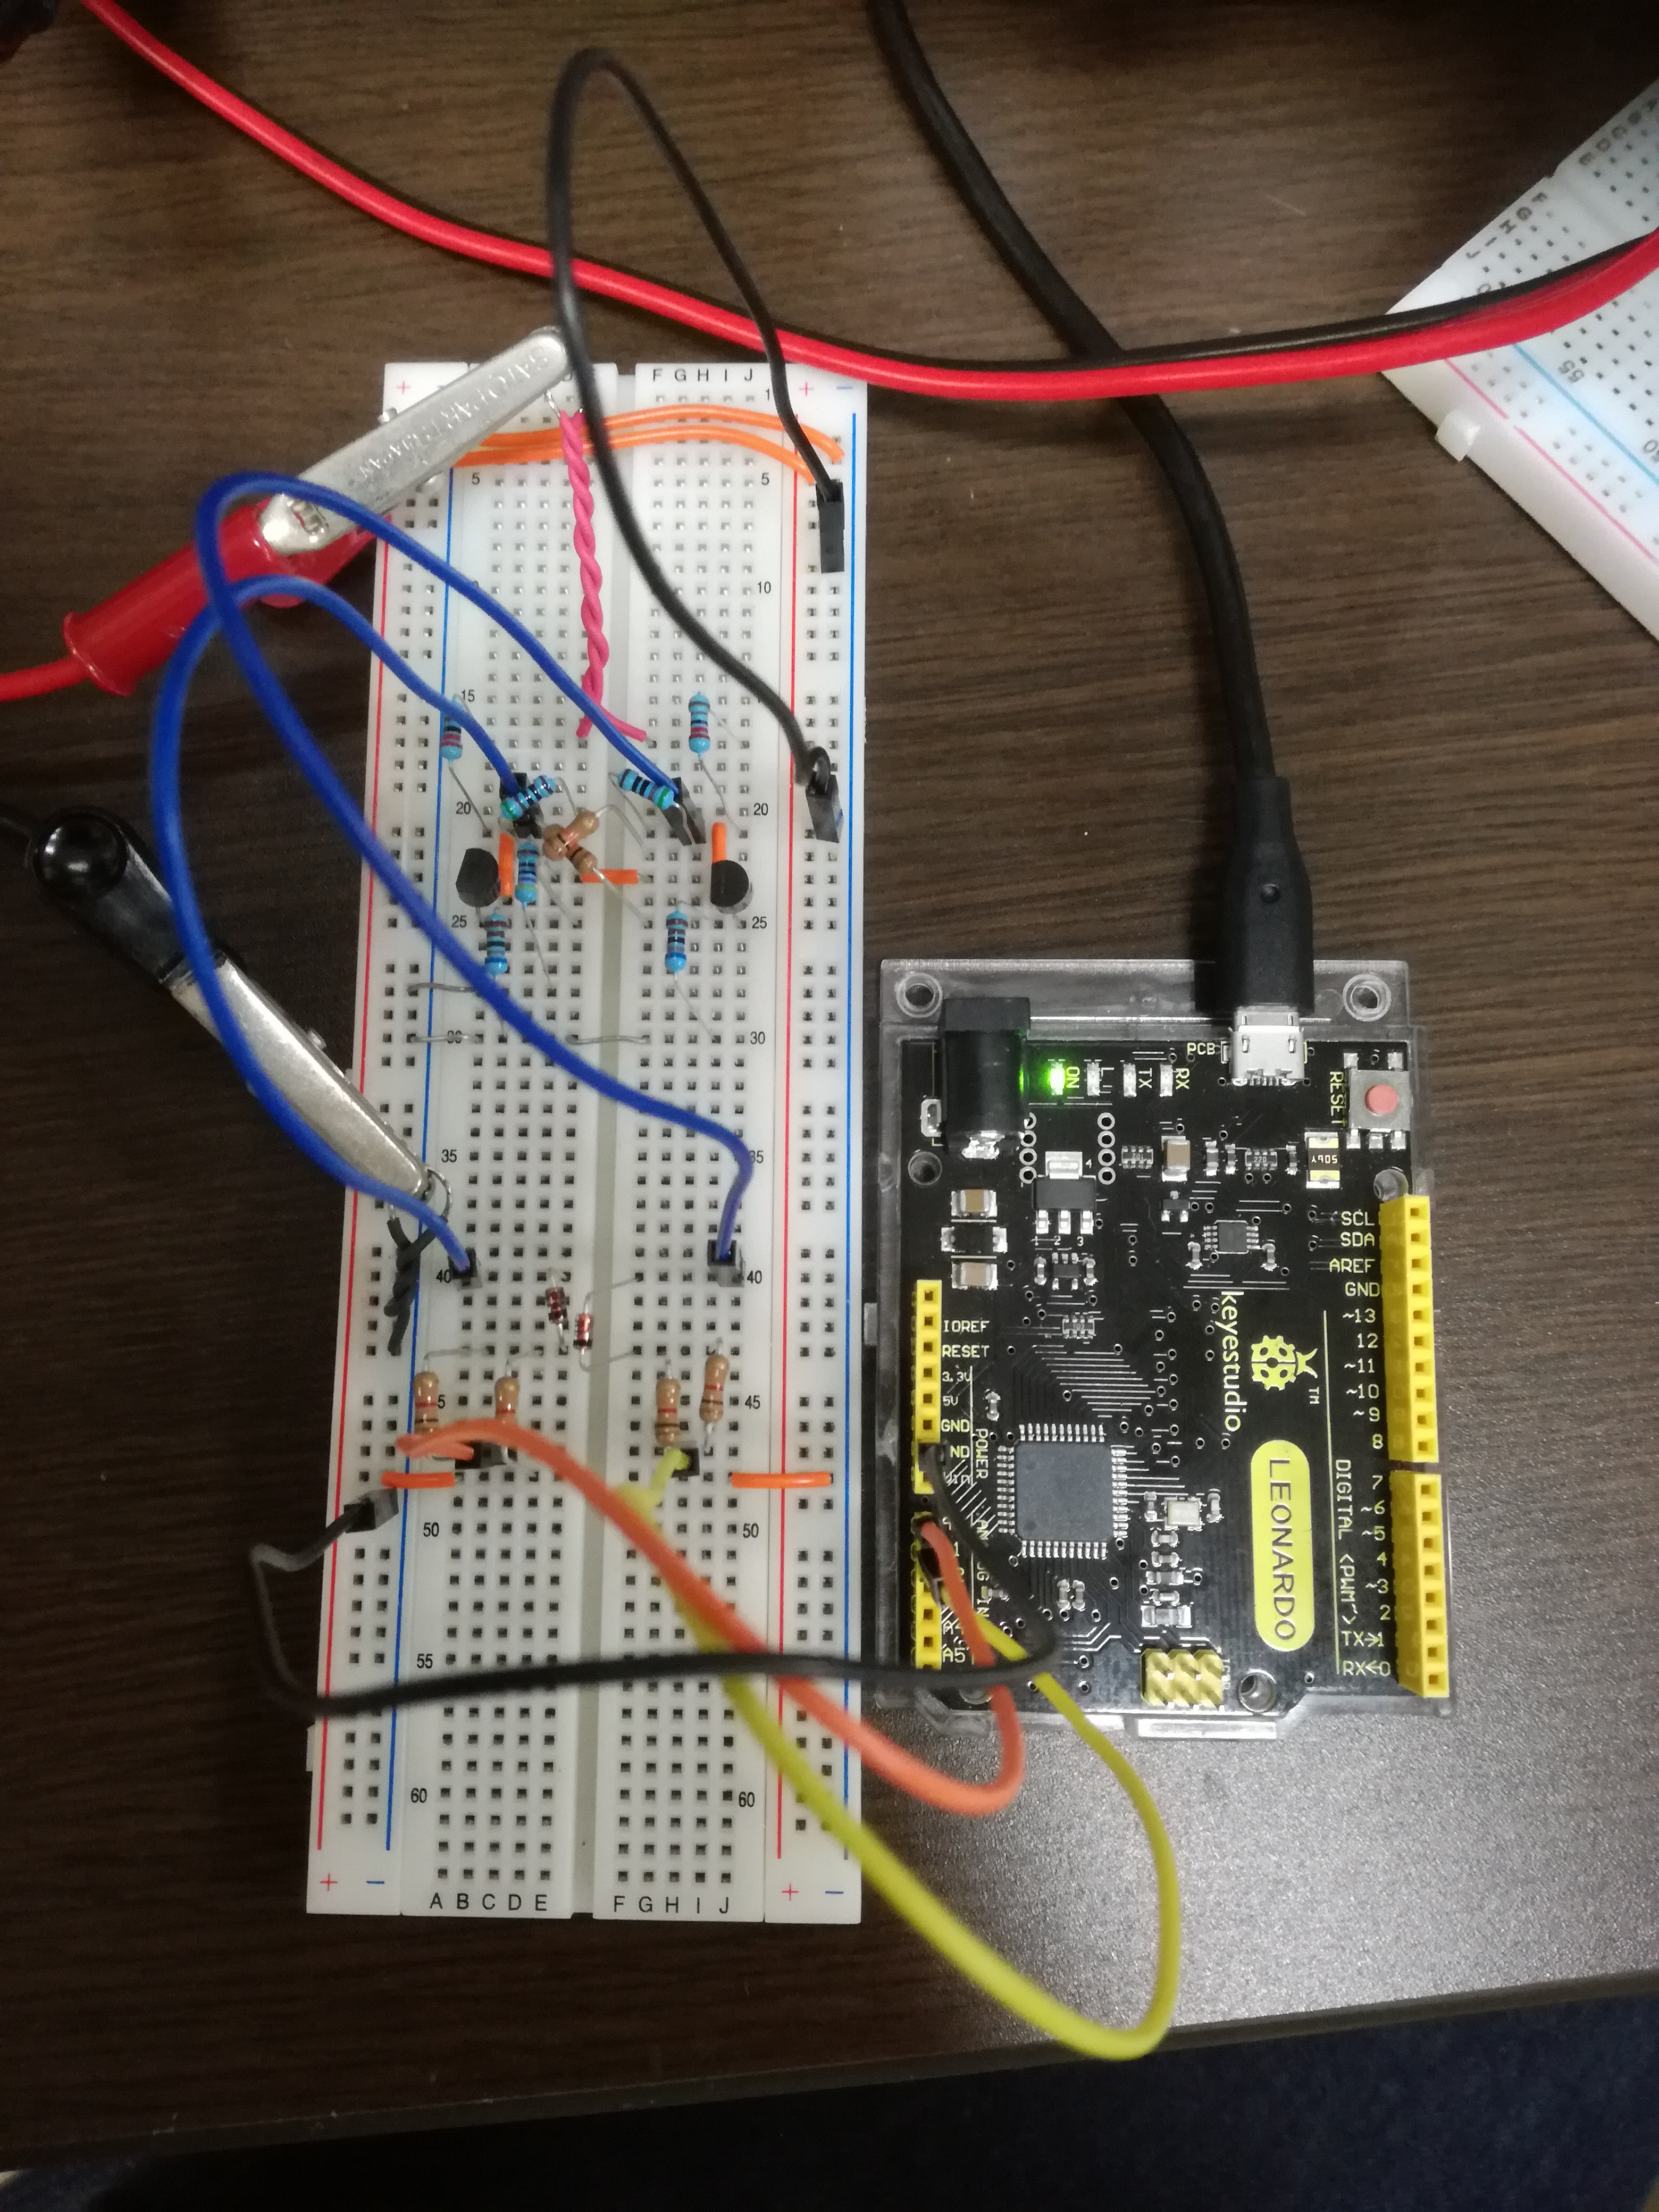
\includegraphics[height=50mm]{images/jisaku-syashin.jpg}
            \caption{制作した回路}
            \label{fig:自作回路写真}
        \end{minipage}
    \end{figure}
    \subsubsection{測定}
    Arduinoに測定用のスケッチをアップロードし,Arduinoから送られてくるシリアル通信のログからグラフを作成し,実験手順4.2の実験の波形の観測を試みた.以下,図\ref{fig:code}にArduinoにアップロードしたスケッチを,図\ref{fig:ex-ex-1}に測定結果のグラフを示す.
    \begin{figure}[H]
        \begin{minipage}{0.5\hsize}
            \centering
            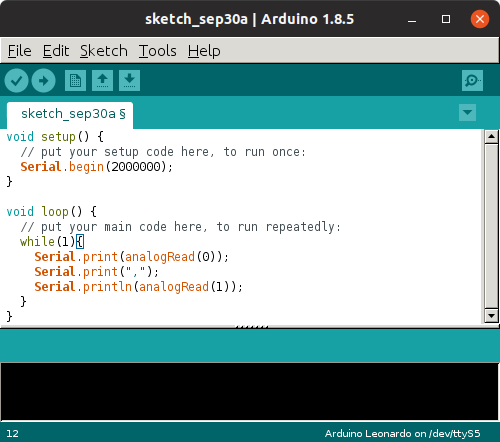
\includegraphics[height=50mm]{images/code.png}
            \caption{使用したスケッチ}
            \label{fig:code}
        \end{minipage}
        \begin{minipage}{0.5\hsize}
            \centering
            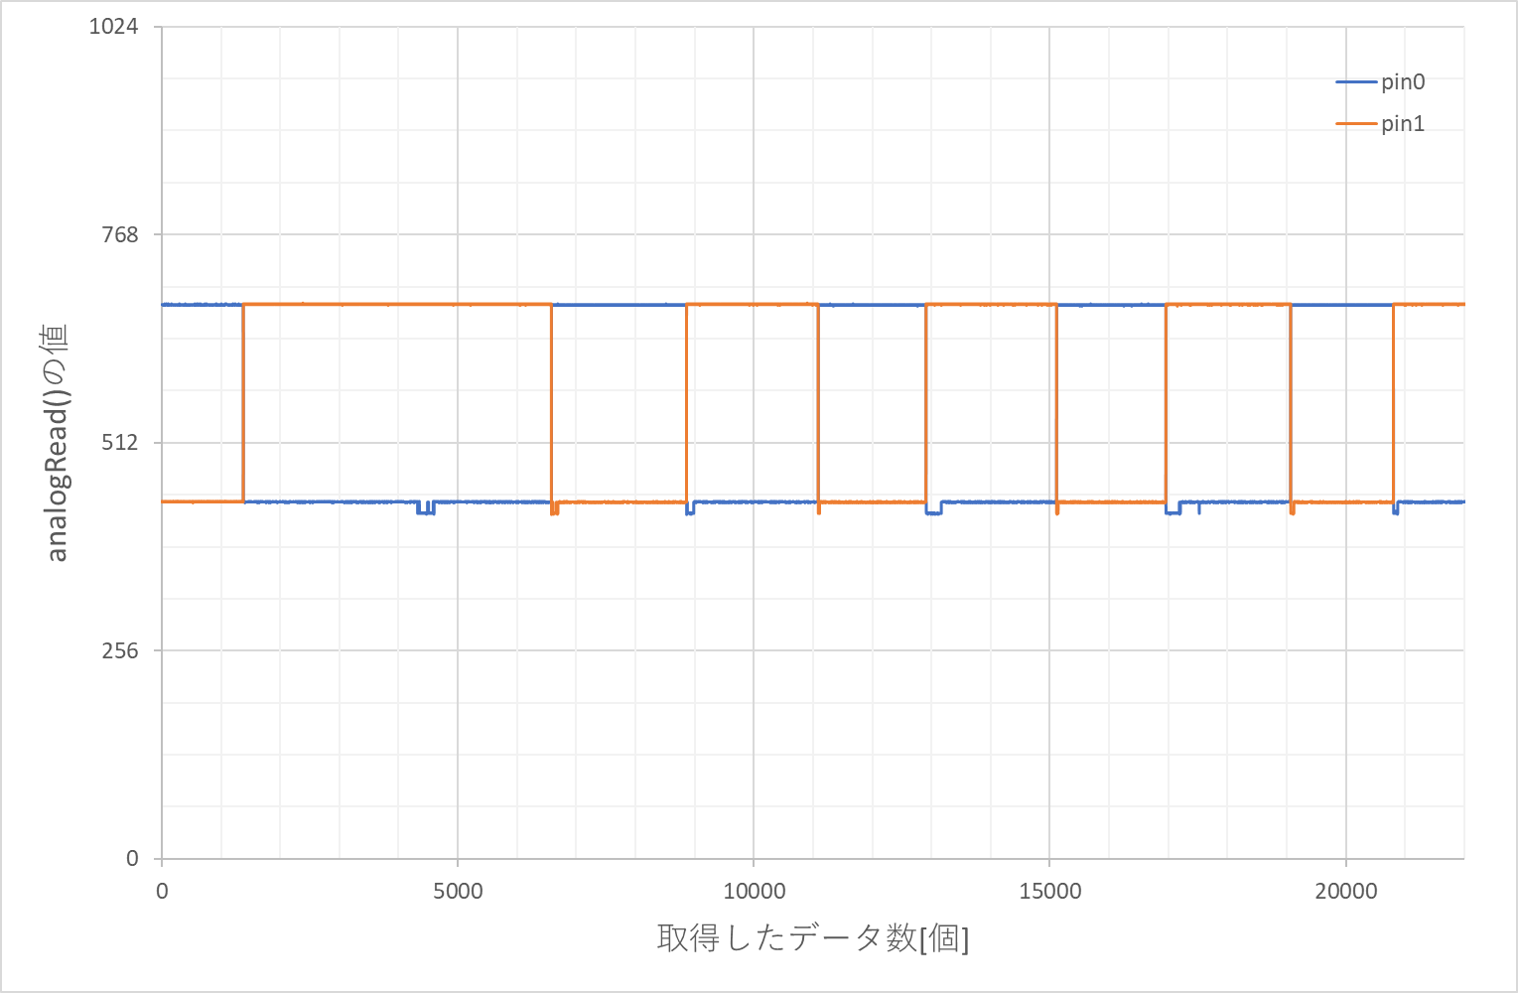
\includegraphics[height=50mm]{images/ex-ex-1.png}
            \caption{制作した回路}
            \label{fig:ex-ex-1}
        \end{minipage}
    \end{figure}
    \subsubsection{結果}
    以上のように,実際に安定状態1と安定状態2が交互に移り変わることが確認できた.

    \section{吟味事項}
    \subsection{スピードアップコンデンサの役割について,実験をもとに考察する.}
    スピードアップコンデンサは,充電されているか否かの状態に応じて,それぞれすばやく電圧を上昇させたり,下降させたりすることが可能であるため,回路の動作がうまく行くと考えられる.

    \section{感想}
    今回,不慮の事故によってデータを紛失してしまったため,波形を測定した実験の結果が全く無い状態になってしまった.今後はデータの管理には万全を期したい.

\end{document}